\documentclass[a4paper,11pt, oneside]{article}  % document class
\usepackage{geometry}
\geometry{
  inner=20mm,
  outer=20mm,
  top=30mm,
  bottom=25mm %
%  heightrounded,
%  marginparwidth=50pt,
%  marginparsep=17pt,
%  headsep=20pt
}
\usepackage[english]{babel}
\usepackage{hyperref}
%pacchetto
\usepackage{import, multicol,lipsum}  % package
\setlength{\columnsep}{1cm}

\usepackage[utf8]{inputenc} % accenti facili
\usepackage[T1]{fontenc}
\usepackage{subcaption}
\usepackage{pifont}
\usepackage{url}
\hypersetup{
	colorlinks=true,
	linkcolor=blue,
	filecolor=magenta,      
	urlcolor=blue
}
\usepackage{graphicx, color, blindtext}
\usepackage{textcomp, makeidx, times}
\usepackage{amsthm, amsmath, amssymb, amsfonts, mathtools} % math
\usepackage[mathscr]{eucal}		
\usepackage[nottoc]{tocbibind} 
\usepackage{pgfplots, parskip}
\usepackage{afterpage, ifthen}
\usepackage{enumitem}
\pgfplotsset{compat=newest}
\usepackage{graphicx} % immagini
\usepackage{wrapfig}
%\graphicspath{ {image/} } % path cartella delle immagini
\usepackage{tikz} %graph
\usetikzlibrary{arrows,automata}
\usetikzlibrary{automata,arrows,positioning,calc,matrix}
\usepackage[linesnumbered,ruled,vlined]{algorithm2e}
\usepackage{booktabs}
\usepackage{colortbl}
\usepackage{siunitx}
\usepackage{tabularx, tabu}
\usepackage{relsize}
\usepackage{makecell, caption, chngcntr}
\usepackage{bbm}
\usepackage{diffcoeff}
\RequirePackage{fix-cm}


%
%____________________________________________________________________________________________________________________________
%____________________________________________________________________________________________________________________________
%____________________________________________________________________________________________________________________________
%____________________________________________________________________________________________________________________________
% INIZIO
\begin{document}

\setcounter{secnumdepth}{2}
\pagestyle{plain} % stile pagina (header, numerazioni)

\centerline {
\includegraphics[width=2cm]{logo.jpg}}
\begin{center}
Università degli Studi di Torino - M.Sc.  in Stochastic and Data Science - A.Y.  2021/2022 \\
\Large { Final project of Statistical Machine Learning (MAT0043)}
\line(1,0){450}\\ 
\vspace{0.4cm} 
{ \huge \textbf{Gene selection for cancer type classification} }
\vspace{0.1cm}
%\hspace{0cm} 
%Group: Bartoli Francesco,  Boetti Chiara, Bordino Alberto (856592)
\line(1,0){450} \\
\end{center}

%____________________________________________________________________________________________________________________________
% ABSTRACT
%In recent years, medicine has made a great step forward in finding new and efficient therapies for different diseases. Thanks to up-to-date technologies, collecting huge amount of data is no longer an issue, so that one can exploit them to define personalised treatments for patients. In particular, cancer genome scale screens are just one example of these applications. In particular, they provide valuable information about the role of genes in driving cancer growth. Thus, researches has developed a Cancer Dependency Map in order to identify genetic and pharmacologic dependencies. However, this is quite a challenging aim: the dataset is not at all easy to handle (high-dimensional, over than $\sim 17.000$ features) and the picked drug-targetable genes should only rely on a specific cancer type, thus imbalanced classes. \\
%In this project, we apply cutting-edge Statistical Machine Learning algorithms to classify different cancer types and select the most relevant genes. After a quick exploratory analysis with PCA, we try Random Forest, Lasso-SVM and Neural Network classifiers and see how the same technique performs differently according to which tumour we are focusing on. In fact, our classification accuracies range from $45\%$ to $98\%$.  \textbf{Aggiungere altre conclusioni}
%\medskip


From the DepMap Portal website, [1], we downloaded a dataset containing 1032 cancerous cell lines whose $\sim 17000$ columns represent the probability that the inhibition of that given gene stops the growth of the cancer.  The label of each cell line refers to the cancer type and is a categorical factor which can assume 9 values: Gastrointestinal,  Gynecologic,  Musculoskeletal,  Neurological,  Breast,  Head-Neck,  Hematologic,  Genitourinary,  Lung.  The project then focuses on the problem of Genes Selection for Cancer Classification,  i.e.  finding a relatively small number of genes to predict the type of cancer of a given tumorous cell.  To this purpose we explored in details three Features Selection algorithms: Random Forests combined with Feature Importance,  Lasso-SVM and Neural Networks (NN) combined with Permutation Importance.  We repeated these procedures on three distinct classification tasks: blood cancer vs rest,  lung cancer vs rest and multiclass.  Apart from the cases involving lung data,  we achieved satisfying classification accuracies on the whole dataset and we were able to select about 100-200 genes from the starting ~17000 ones.  We then fit the reduced versions of those classifier and obtained classification accuracies which range from $67\%$ to $98\%$.  We then concluded that the possibility of classifying the type of cancer from an extremely reduced numbers of genes depends on the cancer type itself.  In particular we observed that blood cancer is the one which separates the most from the other and indeed we achieved almost $100\%$ accuracy using only 100 genes while lung cancer is the worst behaved so this reduced classification task was unfeasible.  In the multiclass task we achieved good classification results with few variables as well and our suspects about lung and blood cancer were confirmed.  


\section{Introduction}
%The mutations that cause cancer cells to grow also confer specific vulnerabilities that normal cells lack. Some of these acquired alterations represent compelling therapeutic targets. The challenge is that, for the overwhelming majority of cancers, we do not fully understand the relationship between the genetic alterations of cancer and the dependencies they cause. To solve this problem, we are creating a “cancer dependency map” by systematically identifying genetic dependencies and small molecule sensitivities and discovering the biomarkers that predict them. \\
Cancer is the uncontrolled growth of abnormal cells anywhere in the body. These abnormal cells are termed cancer cells, malignant cells, or tumor cells.  These cells can  infiltrate normal body tissues. Many cancers and the abnormal cells that compose the cancer tissue are further identified by  the  name  of  the  tissue  that  the  abnormal  cells  originated  from  (for  example,  breast cancer, lung cancer and brain cancer).  When damaged or unrepaired cells do not die and become cancer cells and show uncontrolled division and growth - a mass of cancer cells develop. 
In recent years, medicine has made a great step forward in finding new and efficient therapies for different diseases,  and cancer is one of them.  In particular,   thanks to numerous advances in technology,  collecting huge amount of data is no longer an issue,  so that one can exploit them to define personalized treatments for patients.  An example of this is the DepMap project and,  in particular,  the Achilles project whose aim is to collect data regarding mutations of cancerous cells using genome-wide screens,  identify essential genes and report vulnerabilities across hundreds of human cancers.  \\
Many researches have been done using DepMap datasets and their goal was generally to identify a relatively small number of genes which are responsible for the cancer growth.  The choice of genes is often driven by medical knowledge,  which we do not possess,  together with some rough measure of importance.  Being Maths student we instead based our research only on statistical models and we hypothesized that important genes are the most important features for a given classifier,  where the meaning of "important" will be clarified later.  The implication of selecting a few truly important genes would have outstanding implications in the medical field.  It can be used for example to build faster diagnosis tools or to synthesize less toxic drugs which target a small number of specific genes. 

\section{Dataset}
We use two publicly available datasets, both found on the DepMap Portal website:
\begin{itemize}
	\item \textit{CRISPR\_gene\_dependency.csv}, which contains $1.032$ cancer cell lines characterised by $17.393$ gene scoring results; 
	\item \textit{sample\_info.csv}, which contains cell lines information, such as primary disease and sample collection site.
\end{itemize}
Data were collected from real patients and successively processed, so that each element of this $(1.032 \times 17.393)$-matrix is the probability that knocking out a gene has a real depletion effect on the cell. \\
First of all, we look for any missing values: only 10 rows have empty columns, specifically either $678$ or $1.285$ Nas. At first impact, this could seem a big deal, but it is actually the $4\%$ and $7\%$  of the total genes. Moreover, these cells come from different tumours, so we decide to simply remove them all.  \\
Before proceeding with our analysis, we also notice some weird observations: $2$ of them are labelled as "Non-Cancerous" and $6$ as "Engineered". The first can be reasonably discarded as our goal is classifying cancer cells, whereas the latter requires a little care. Engineered cells are synthetically modified sample in lab and, here, they are manly associated to the Eye sample collection site. We keep them and we associate the cancer type according to the sample. \\ \\
One could ask: why do we focus only on the primary disease and not also on the sample collection site, as done for Engineered observations? If we count the number of cells with respect to cancer type and collections site, we find many peculiarities. For instance, some Brain-cancer cells have been picked from the abdomen, whereas Lung-cancer cells comes from a variety of different places. This is because of the nature/curse of cancer: metastasis are ill cells identifiable as the original tissue but found on a different site. Therefore, this subdivision would only complicate our task. 

\begin{wrapfigure}{r}{0.65\textwidth}
	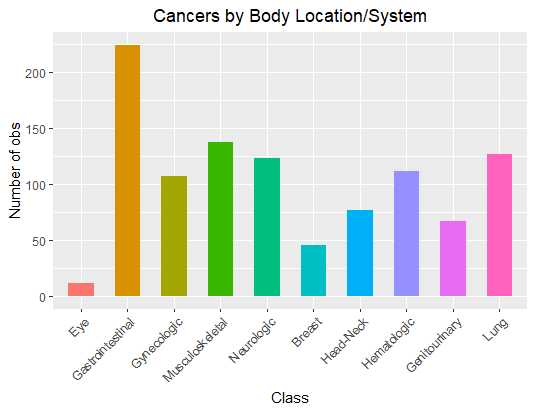
\includegraphics[width=0.65\textwidth]{Rplot-classes.png}
	\captionof{figure}{Cancer classes}\label{fig1}
\end{wrapfigure}
We group the various cancer types in 10 classes according to common medical knowledge, [4], and we obtain the classes as reported in Figure \ref{fig1}. \\
We see that class "Eye" is the smallest one: there are only $16$ observations and $5$ of them are labelled as Enginereed, previously referred as \textit{weird observations}. On the other hand, "Gastrointestinal" is the largest class and it comprehends $7$ types of cancer, making this group quite dispersive. We hence grasp that these two classes could cause some problems in classification. \\
Still following our intuition, we decide to focus our One-Vs-All binary classification on the "Lung" class. Since all these samples have been originally labelled as lung tumours, we suppose they do not suffer from noise caused by grouping together different disease. \\
On the other hand, we choose to study the "Hematologic" group relying on some underlying biological knowledge. In fact, Blood cancer is quite different from other tumours because:
\begin{itemize}
	\item blood is in the whole body, and so the cancer is, too;
	\item Leukemia, Lymphom and Myeloma are the main kinds of cancer but they all effect white blood cells;
	\item not all blood cancers require a treatment, just periodical monitoring.
\end{itemize} 


\section{Methods}


\section{Results}


\section{Conclusion and future works}


%\end{multicols}

\begin{thebibliography}{11}   % BIBLIOGRAFIA
% \bibitem{Baum} L. Baum, T. Petrie, \textit{Statistical Inference for Probabilistic Functions of Finite State Markov Chains}, in Ann. Math. Stat., 37, 1554-1563, 1966 \\
\bibitem{DepMap} DepMap Portal: \url{https://depmap.org/portal/}  \\
\bibitem{DepMapData} DepMap, Broad (2021): DepMap 21Q3 Public, figshare. Dataset: \url{https://doi.org/10.6084/m9.figshare.15160110.v2} \\
\bibitem{Achilles} Project Achilles: \url{https://depmap.org/portal/achilles/}  \\
\bibitem{Classes} Cancer types grouped by body location: \url{https://www.cancer.gov/types/by-body-location} \\
\end{thebibliography}
\end{document}